%In this section, the layer is described in some detail in terms of its specific subsystems. Describe each of the layers and its subsystems in a separate chapter/major subsection of this document. The content of each subsystem description should be similar. Include in this section any special considerations and/or trade-offs considered for the approach you have chosen.
In this section, we describe the move decision layer. This layer is responsible for the decision making process of the UR5 robot for the Checkers game.
\subsection{Artificial Intelligence}
%This section should be a general description of a particular subsystem for the given layer. For most subsystems, an extract of the architectural block diagram with data flows is useful. This should consist of the subsystem being described and those subsystems with which it communicates.
The Artificial Intelligence communicates with the camera and Computer layer subsystems to make decisions for the UR5 robot arm.
\begin{figure}[h!]
	\centering
 	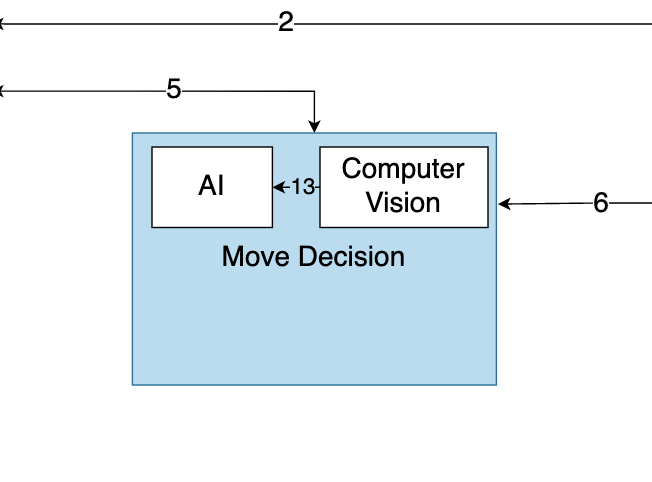
\includegraphics[width=0.60\textwidth]{images/Screenshot 2022-11-13 at 6.09.50 PM.png}
 \caption{Move decision layer subsystems diagram}
\end{figure}

\subsubsection{Assumptions}
%Any assumptions made in the definition of the subsystem should be listed and described. Pay particular attention to assumptions concerning interfaces and interactions with other layers.
N/A

\subsubsection{Responsibilities}
%Each of the responsibilities/features/functions/services of the subsystem as identified in the architectural summary must be expanded to more detailed responsibilities. These responsibilities form the basis for the identification of the finer-grained responsibilities of the layer's internal subsystems. Clearly describe what each subsystem does.
The Artificial Intelligence calculates the next move for the Computer. It compares the best move by looking at the next two to three steps ahead by the appropriate algorithm. It also determines any invalid moves by the player.  

\subsubsection{Artificial Intelligence Interfaces}
%Each of the inputs and outputs for the subsystem are defined here. Create a table with an entry for each labelled interface that connects to this subsystem. For each entry, describe any incoming and outgoing data elements will pass through this interface.
Details in Table 5 show the incoming and outgoing data elements.
\begin {table}[H]
\caption {Subsystem interfaces} 
\begin{center}
    \begin{tabular}{ | p{1cm} | p{6cm} | p{3cm} | p{3cm} |}
    \hline
    ID & Description & Inputs & Outputs \\ \hline
    \#5 & Signal from the computer & \pbox{3cm}{N/A} & \pbox{3cm}{N/A}  \\ \hline
    \end{tabular}
\end{center}
\end{table}

\subsection{Computer Vision}
%This section should be a general description of a particular subsystem for the given layer. For most subsystems, an extract of the architectural block diagram with data flows is useful. This should consist of the subsystem being described and those subsystems with which it communicates.
The Computer Vision interacts with the frames received from the camera to determine the player's move.

\subsubsection{Assumptions}
%Any assumptions made in the definition of the subsystem should be listed and described. Pay particular attention to assumptions concerning interfaces and interactions with other layers.
N/A

\subsubsection{Responsibilities}
%Each of the responsibilities/features/functions/services of the subsystem as identified in the architectural summary must be expanded to more detailed responsibilities. These responsibilities form the basis for the identification of the finer-grained responsibilities of the layer's internal subsystems. Clearly describe what each subsystem does.
It successfully identifies the movements of the Checkers pieces. It also identifies the current locations on the Checkers board.

\subsubsection{Subsystem Interfaces}
%Each of the inputs and outputs for the subsystem are defined here. Create a table with an entry for each labelled interface that connects to this subsystem. For each entry, describe any incoming and outgoing data elements will pass through this interface.
Details in Table 6 show the incoming and outgoing data elements.
\begin {table}[H]
\caption {Computer Vision interfaces} 
\begin{center}
    \begin{tabular}{ | p{1cm} | p{6cm} | p{3cm} | p{3cm} |}
    \hline
    ID & Description & Inputs & Outputs \\ \hline
   \#13 & Send input to Artificial Intelligence & \pbox{3cm}{Computer Vision input} & \pbox{3cm}{Checkers Move}  \\ \hline
    \#6 & Receives camera frames & \pbox{3cm}{Camera Frames} & \pbox{3cm}{Checkers board movement}  \\ \hline
    \end{tabular}
\end{center}
\end{table}